% Use a modified ACM conference proceedings template
\documentclass[sigconf]{acmart}
% Disable some elements from ACM template
\setcopyright{none}
\settopmatter{printacmref=false,printfolios=false}

\usepackage{booktabs} % For formal tables
\usepackage[ruled,vlined]{algorithm2e} % for writing algorithms

\begin{document}
\title{Machine Perception Report}

\author{Fatjon Zogaj}\affiliation{}
\email{fzogaj@student.ethz.ch}

\author{Patrik Okanovic}\affiliation{}
\email{pokanovic@student.ethz.ch}

\author{Rafael Sterzinger}\affiliation{}
\email{rsterzinger@student.ethz.ch}

\begin{abstract}
%Briefly summarize your report here. This should include a description of the task you are solving, a summary of how you approach the task (i.e. your method), as well as a preview of the central result. The abstract should be short, i.e. 4-5 sentences. The rest of this template outlines a rough structure how you \emph{can} organize your report. It mentions all the components we would typically expect. It is a good idea to adhere these guidelines, but they are not binding, i.e., you are free to re-organize your report as you see fit.
\end{abstract}

\maketitle

\section{Introduction}
%In this section, introduce the task in a bit more detail. In the first paragraph, try to answer why the task is of interest at all and what makes it challenging. You may also discuss some related work here. For example, you can summarize how other researchers have addressed the problem and what might be the disadvantages of these works.

%In the second half of the introduction, describe your method. This should be more detailed than in the abstract. You can talk about how your method relates to existing work (e.g. it is a combination or extension of existing methods, what other papers were you inspired by, etc.). You should also state the central result here, and the key insight that made it possible to achieve this result.

Human pose estimation (HPE) from a single monocular image is an open challenge garnering significant attention in computer vision ~\cite{DBLP:journals/corr/PavlakosZDD16} as it offers a wide variety of useful applications in real-life.
For instance, HPE is utilized in human tracking, human-computer interaction, sports motion analysis, and self-driving cars ~\cite{chen_monocular_2020}.
Estimating the full-body pose has been extensively studied in both 2D and 3D ~\cite{sun_compositional_2017}.
Thanks to the availability of large-scale 2D annotated human poses and the emergence of deep neural networks achieving very low error rates~\cite{yang2020transpose, bulat2020skip, su2019multi}, the 2D human pose estimation problem is considered as nearly solved.
In contrast, the 3D human pose estimation remains an open problem.
This is partially because of the ambiguity of recovering the 3D information from single images and also due to the lack of large-scale 3D pose annotated datasets.
Methods for solving the 3D human pose estimation can roughly be divided into two categories:
i) learning end-to-end networks that recover 2D input images to 3D poses directly,
ii) extracting 2D human poses from input images and then lifting 2D poses to 3D
spaces~\cite{DBLP:journals/corr/abs-1710-06513}.

One of the drawbacks of learning end-to-end or regressing directly \todo{check this}, is that the per-joint location errors are minimized independently ignoring the internal structure.
Decoupling \todo{*D} HPE into 2D and 3D part has some advantages.
With decoupling one can make use of the existing large-scale 2D pose estimation datasets.
Additionally, infinite 2D-3D pairs can be generated using different projections and similar techniques ~\cite{DBLP:journals/corr/abs-1710-06513}.
However, in order to optimize these models, further supervision in various forms is required, such as camera parameters in multiview settings ~\cite{DBLP:journals/corr/abs-1903-02330}.


%\section{Related Work}
%\todo{This section is optional and it is fine to leave it out completely. While the most relevant papers should be discussed adequately somewhere (e.g. in the introduction), we do not expect you to give a complete overview of related work. Nonetheless, if you would like to do so, this would be the place to do it.
%
%Generally, use the \texttt{{\char'134}cite} command to cite other works, e.g. \cite{Douglass98,Harel79}. To add a new reference, you need to add a bibtex entry to the bibliography file, in this case \texttt{bibliography.bib}.
%}


\section{Method}
This section describes the methods used in our final model which includes e.g. preprocessing steps, augmentations, changes of representation, parameters, and the architecture of the model.
%This section should describe the method of your \emph{final} submission in detail. This includes things you did with the data (e.g. preprocessing, augmentations, changes of representation, etc.) and the actual definition of your model. Sometimes it is fine to describe a model in text or math only, sometimes it is better to create an overview figure. Either way, after reading this section, a reader should be able to implement your architecture.
%If you have enough space, you may list hyperparameter values in an ``Implementation Details'' paragraph. Otherwise list them in the README of your code repo.

\subsection{Data augmentation}
Despite the success of deep models, many of them are still data-hungry, therefore we augmented our given dataset to satisfy this hunger.
The input pictures are normalized to 284 x 284 dimension \todo{and patched to a size of 256 x 256 dimensions/288 x 384 dimensions} TODO. Standard data augmentation includes rotation $\pm 30$ degrees, horizontal flipping, scaling by a factor between $0.75$ and $1.25$, and color scaling between $0.8$ and $1.2$.
Overall, frames are rotated with a probability of 60\% and flipped with a probability of 50\%.

\subsection{Data occlusion}

Furthermore, we use synthetic occlusion to make the network robust to occluded joints, since erasing objects or simply putting them in the picture improves results in image classification, object detection, and person identification~\cite{sarandi_synthetic_2018}.
Using objects from the Pascal VOC dataset we filter out persons, segments with area below 500px and segments labeled as \emph{difficult} or \emph{truncated}.
Finally, with the defined probability \todo{$p_{occ}$} a random number between 1 and 8 of objects from the filtered VOC dataset are added to random locations of the frame.

\subsection{Backbone Model}
\todo{Pre-trained model, ResNet and its variations in general, layer freezing, final head}

\subsection{Heatmap Regression}

Another important development in the task of HPE was the introduction of heat map representations as an alternative to directly regressing the joint locations.
In this representation each location in the heat map represents a probability of the joint being at this position ~\cite{sun_integral_2018-1}.
Given such a heat map representation $\mathbf{H}_k$ for the $k^{th}$ joint, the position of the joint $\mathbf{J}_k$ is estimated by the maximum likelihood

$$\mathbf{J}_k=\underset{\mathbf{p}}{\text{argmax}}\ \mathbf{H}_k(\mathbf{p})$$

In our case, such a heat map representation is learnt by a shallow head from extracted convolutional features from our backbone.
This head network consists of 3 deconvolution layers which upsample the extracted features to a certain resolution (64 x 64 by default) which are then followed by a final convolution layer that produces $K$ heat maps.
For almost all of our experiments we used 64 heat maps per joint, however, as this value directly corresponds to the granularity of the z-dimension, we later increased this value to 72.

This approach yields good performance in HPE but has two clear drawbacks compared to directly regressing the join locations.
The first one is the usage of the \textit{argmax} operator that makes the calculation of the maximum likelihood non-differentiable which hinders the possibility of training a neural network end-to-end.
The second drawback is a quantization error which stems from down sampling steps performed by the backbone.
\citeauthor{sun_integral_2018-1} {\cite{sun_integral_2018-1}} alleviate these problems by modifying the joint calculation to "taking-expectation" instead of "taking-maximum".
With this, the above equation in the discrete case can be formulated as
$$\mathbf{J}_k = \sum_{p_x=1}^D\sum_{p_y=1}^H\sum_{p_x=1}^W\mathbf{p}\cdot \mathbf{H}_k(\mathbf{p})$$
which is also known as the \textit{soft argmax}.
This formulation can further be modified which then allows to calculate the expected joint position in each dimension separately.
A benefit from this is the additional option to train on 2D (MPII) and 3D (H36M) data simultaneously and end-to-end.

Given the fact that the first \cite{sarandi_synthetic_2018} and second \cite{sun_integral_2018} place of the 2018 ECCV PoseTrack Challenge made use of this heat map representation with the \textit{soft argmax}, we employed this technique as well.


\section{Other Approaches}
In the following section we list different techniques which
performed similarly or worse than the ones included in the presented best model.

\subsection{Graph Neural Networks}
As the task of 2D human pose estimation has been extensively studied, achieving very low
error rates~\cite{yang2020transpose, bulat2020skip, su2019multi},
also take a look at an architecture for 3D-joint regression based on 2D-joint input.
A human skeleton follows the underlying structure of a graph which is why a
Graph Convolutional Network (GCN) offers itself well to model this.
Making use of \citeauthor{zhao2019gcn}'s Semantic GCN (SemGCN) model allows us to capture semantic
information in regard to global and local joint relations~\cite{zhao2019gcn}.

As the original SemGCN model utilizes joint grouping (maxpool: 16 joints \textrightarrow ~8 joints), we adapt it for
our use case of 17 joints.
We have looked at a variety of ways on how to incorporate the missing joint (Neck/Nose).
These options include:
\begin{itemize}
    \item simply concatenating the missing joint to the other grouped ones
    \item grouping the missing joint with itself
    \item grouping the missing joint with other related joints
    \item removing grouping altogether
\end{itemize}
We also played around with reordering the joints to put more emphasis on one over another
as max-pooling makes use of locality.

Two different training approaches offer themselves well for this.
In the first one the training of the SemGCN can be separated into two parts.
We first train the SemGCN to predict the z-axis based on 2D ground truth input data.
Afterwards we use this pre-trained model and stack it on top of our also pre-trained backbone,
dropping the third dimension of the backbone output to feed it into the SemGCN.
The second approach simply stacks the untrained SemGCN on top of the backbone and trains it
together from scratch.

On top of that we differentiate between the case of freezing the backbone model completely, and only
freezing its last layer and respective head.

\subsection{Evolutionary Training Data}
Finally, in order to train the mapping of joints from 2D to 3D we have used an evolutionary technique for augmenting the dataset as proposed in ~\cite{Li_2020_CVPR}. In order to implement the evolutionary data augmentation, joints of the human 3D skeleton are represented by a set of bones organized hierarchically in a kinematic tree, this way the dependence of adjacent joints with tree edges is captured. This can be seen in Fig. ~\ref{skeleton}. Assuming that $\textbf{p}^j$ is the \emph{j}-th joint and \emph{parent(i)} returns the parent joint index of the \emph{i}-th bone vector, then each pose \textbf{p} corresponds to a set of bone vectors $\{\textbf{b}^i\}_{i=1} ^{w}$ and every bone vector is defined as

$$\textbf{b}^i = \textbf{p}^{child(i)} - \textbf{p}^{parent(i)}$$

%\begin{figure}
%    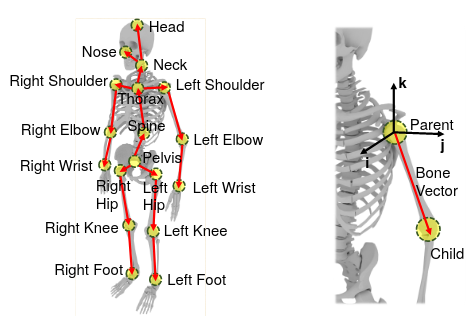
\includegraphics[height=4cm, width=7cm]{skeleton.png}
%    \caption{\todo{remove if > 3 pages} Hierarchical human representation. Left: 3D key-points organized in a kinematic tree where red arrows point from parent joints to children joints. Right: Zoom-in view of a local coordinate system, source ~\cite{Li_2020_CVPR}}
%    \label{skeleton}
%\end{figure}

Every parent node has attached a local coordinate system which can be seen in Fig. ~\ref{skeleton}. For $\textbf{p}^{parent(i)}$ local coordinate system is represented by the rotation matrix $\textbf{R}^i = [\textbf{i}^i, \textbf{j}^i, \textbf{k}^i]$, which is used to transform the bone vector into the local coordinate system with the following equation:

$$\textbf{b}_{local} ^{i} = \textbf{R}^{i\textbf{T}}(\textbf{p}^{child(i)}-\textbf{p}^{parent(i)})$$

which is for convenience transformed into spherical coordinates $\textbf{b}_{local}^i = (r_i, \theta _i, \phi _i)$.

The overall algorithm can be seen in ~\ref{alg1}.

\begin{algorithm}
    \SetKwInOut{Input}{input}
    \Input{Initial population of 3D joints $D_{old}=\{\textbf{p}\}_{i=1} ^N$, noise $\sigma$, number of generations $G$}

    $D_{new} = D_{old}$

    \For{i=1:G}{
    Parents=Sample($D_{new}$)

    Children=NaturalSelection(Mutation(Crossover(Parents)))

    $D_{new} = D_{new} \cup Children$
    }
        return $D_{new}$
        \caption{Data evolution}
        \label{alg1}
\end{algorithm}

With algorithm ~\ref{alg1} we create 2D-3D pairs for learning the model to map from 2D to 3D. Since the data is represented as we mentioned in a hierarchical way crossover is intuitive to implement. Crossover is implemented as a random exchange of sub-trees. TODO: do we want the formal definition?. Mutation operator pertubates the local orientation of one bone vector. Bone vector $\textbf{b}_i = (r_i, \theta _i, \phi _i)$ is randomly selected and Gaussian noise $g ~ N(0, \sigma)$ is added

$$\theta _i ' = \theta _i + g_{\theta}, \phi _i ' = \phi _i + g_{\phi}$$

Mutation can easily make an invalid pose, therefore we use natural selection to remove invalid poses. Natural selection is implemented using a function $v(\textbf{p})$ which indicates which pose is invalid and gives that pose a value of $-\infty$ making it unable to be selected into the new generation. This function uses the prior angle constraints defined from ~\cite{Akhter_2015_CVPR}.
Both mutation and crossover can be seen in Fig. ~\ref{evolved}

\begin{figure}
    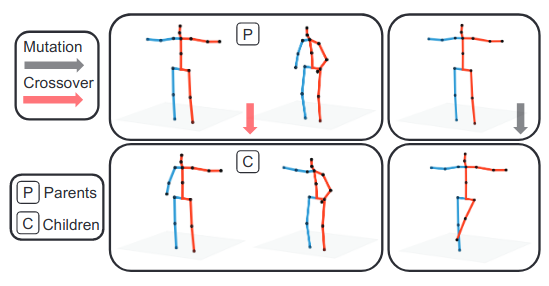
\includegraphics[height=5cm, width=8.5cm]{evolution.png}
    \caption{Examples of evolutionary operation. Crossover and mutation take two and one random samples respectively to synthesize novel human skeletons. In this example the right arms are selected for crossover while the left leg is mutated., source ~\cite{Li_2020_CVPR}}
    \label{evolved}
\end{figure}

\subsection{Miscellaneous}

In addition to the approaches above, we have combined them with a variety of further techniques.
As the official PyTorch documentation recommends loading in the data in the range of [0, 1],
we have tried [0, 1]-normalization instead of the original z-standardization.
Preliminary experiments showed that this does not improve the score, hinting at a slight decrease
which is why it was not further used.

Furthermore, although ensemble methods were not allowed, using dropout layer were an exception.
Hence, we have experimented using a dropout layer after the heatmaps \todo{and after the freature extraction part}, however it did not \todo{improve our score} give a better score than our best model.

Before evaluating the SemGCN architecture to lift our 2D joint predictions to 3D, we explored the idea of utilizing a de-noising autoencoder as a refinement step to our 3D joint predictions.
We borrowed this idea from the authors \citeauthor{ghosh_learning_2017} \cite{ghosh_learning_2017} which use this component to adjust unfeasible poses from human motion predictions.
After some testing of this idea, we learned about the SemGCN architecture which seemed more promising and hence stopped further exploration.

After initial test runs of the SemGCN architecture, we noticed a bottleneck stemming from our 2D joint predictions when compared to training on the ground truth 2D H36M data.
As we previously simply dropped the last axis of our 3D predictions to create the 2D input, we thought if we train the backbone to predict 2D joint locations only, accuracy might improve.
Having tried both methods with not improvement in accuracy, we conclude that there is no performance gain in varying these approaches.

\todo{bone loss}
Both of the just mentioned ideas focus more or less on capturing the overall human pose composition.

\todo{whats up with this part?}
Exploiting GCN's resemblance to the human skeleton, a comparison is also made between using 2D and 3D joints as input data.
In the latter case the SemGCN would act as a final refinement step.



\section{Evaluation}
We evaluate models for 10 to 30+ hours, starting with a learning rate of 0.0001 and reducing it by 10
after 90 and 120 epochs or manually after a 10 hour run if the loss seems to have converged. \todo{maybe move to Method?}
\todo{In the evaluation section you should describe the experiments that support the claims of the story of your report. For example, if you previously said ``We propose to combine model A with component B which leads to improved accuracy.'' you should back this up with experimental evidence here. Typically, this means that you should show the performance of model A with and without component B. May be your method warrants other kinds of such ablation studies, which you might include and describe here.}

% 55 epochs on both 50/50 then smaller lr only on h36m

\begin{table}[h!]
    \caption{Ablation study on the progression of the Mean Per Joint Position Error (MPJPE) metric. The score denotes the performance on the test set. Values with $*$  denote the performance on the validation set.
    Data occlusion (O), Data augmentation (A), Integral Heatmap Regression (I), Extra Data (E),
    3D-Regression (R), Higher Resolution (H), Bone Loss (B), %Backbone Completely Frozen (C),
    Last Layer Unfrozen (U), Remove Joint Grouping (G), 3D SemGCN Input (3), Ground Truth Pre-Training (P),
    SemGCN Head (S)
    \todo{order these by alphabet for easier finding\\ i would also have the first part of the ablation study be steadily decreasing in performance and move expereiments which were not submitted to the end}
    }
    \label{tab:ablation}
    \centering
    \begin{tabular}{|| c | c | c ||}
        \hline
        \textbf{Backbone} & \textbf{Extensions} & \textbf{MPJPE}$_{test}$      \\
        \hline\hline
        AlexNet           & R                   & 141.50                       \\
        \hline
        AlexNet           & O                   & $84.50_{\downarrow 40.28\%}$ \\
        \hline
        ResNet50          & I                   & $72.15_{\downarrow 49.01\%}$ \\
        \hline
        ResNet50          & I,O                 & $63.01_{\downarrow 12.69\%}$ \\
        \hline
        ResNext101        & I,O,A               & $54.14_{\downarrow 14.08\%}$ \\
        \hline
        ResNext101        & I, O, A, S, 3       & $57.43$                      \\
        \hline
        ResNet152         & I,O,A,H,E           & $50.94$                      \\
        \hline
        ResNext101        & I,O,A,H,E           & $48.95$                      \\
        \hline
        ResNext101        & I,O,A,B             & $54.60^*$                    \\
        \hline
        SemGCN            &                     & $66.87^*$                    \\
        \hline
        SemGCN            & P                   & $60.08^*$                    \\
        \hline
        SemGCN            & P, U                & $54.12^*$                    \\
        \hline
        SemGCN            & P, U, G             & $46.05^*$                    \\
        \hline
    \end{tabular}
\end{table}

\textbf{Effect of synthetic occlusion}: using the given sample code with the AlexNet as the backbone of the model synthetic occlusion gives an impressive improvement to the score lowering it for 40.28\%.

\textbf{Effect of model backbone}: stronger backbone plays a significant role when it comes to improving the score. Using the ResNet50 with integral heatmap regression improved the score from the initial model for 49.01\% adding synthetic occlusion to that gives a score which has 12.69\% lower MPJPE on the test set. Furthermore, using even more powerful backbone such as ResNext101 with integral heatmap regression, synthetic occlusion and standard augmentation improved the model to a score of 54.14 MPJPE. One can compare using ResNext101 to ResNext152 with identical extensions as shown in ~\ref{tab:ablation} to see that ResNext101 gets a score better for 3.91\%, this can be explained : \todo{explain}

\textbf{Effect of larger image size/depth resolution}: \todo{larger image and additionaö set into one category? not separated in the scores?}

\textbf{Effect of additional validation set}:

\subsubsection*{SemGCN}
\todo{change everything to stringent flow of End-to-End or SemGCN only}
In regards to the SemGCN model, only the scores of the z-axis matter as the other 2D input is the ground truth.
Thus, the following error scores for the SemGCN are not directly comparable to the others.

Our first experiments showed that when not pre-training the SemGCN model on ground truth data,
it is able to achieve a validation score of 66.87.
This can be brought down to 60.08 by incorporating pre-training.
%The best variant making use of pre-training on ground-truth data achieves a validation error of 54,
%while not pre-training achieves 66.

As a next step we then analyzed the effect of unfreezing the last layer of the backbone which
achieves a score of 54.12.
Unfreezing the SemGCN without any pre-training on the other hand got an error of around 65.5.
This could be explained due to the fact that we stop training the model if it seems to perform badly
early on, which is the case for non-pre-trained models as these take longer to train.
%This best pre-trained SemGCN leaves the last layer unfrozen, while freezing
%the backbone completely achieved a validation error of 60.08 when using a pre-trained model.

Like previously mentioned, we compare different ways of adding the missing 17th joint,
ranging from simple concatenation and group removing
to more sophisticated grouping with other joints and reordering.
Surprisingly the grouping methods even in combination with joint reordering perform similarly bad
with scores around 60 using pre-trained models.

Removing the grouping altogether seems to prove most useful, being able to get a validation error of 46.05.
This holds for the case where we change the architecture to not consider grouping as well as when
we simply change the group size to 1 instead of 2.
This might be explained due to the model's robustness
and the possibility that few of the joints make up for most of the information lying underneath.

\todo{I'd just leave out going into detail for End to End Models selling it as the same thing for both
and maybe in passing mention that we did not
validate them all too much as the SemGCN didn't perform too well already.
Or we can have SemGCN (S) as an extension for the ablation study and add it under ResNext}


\section{Discussion}
In this section we give possible explanations as to why some approaches fared better
than the other and which mechanisms could lie behind.


\todo{Sometimes you might have had a great idea, but it did not pan out. Since we want to encourage novelty, such failed attempts should also go into the report. This section is a suitable place to discuss this. If you can, do not just list failed attempts, but actually \emph{discuss} them, i.e., provide an intuition why you think they failed or what the problem is that prevented them from performing better. It is much better to describe one failed attempt and discuss it in-depth than just listing four failed models without any explanation.

If you do not have failed attempts that would warrant their own section, this is perfectly fine. You may discuss the experiments from the previous section here, or if you prefer to have the discussion the evaluation section directly, feel free to omit this section entirely.}


\section{Conclusion}
%Conclude your report with a brief summary. This can be very short, i.e. 2-3 sentences.
In this paper we compare a variety of different architectures and techniques for the
task of 3D human pose prediction on the H36M dataset \cite{h36m_pami}.
We provide an extensive benchmark study analyzing direct image-to-3D-joint prediction
as well as image-to-2D-joint prediction with a final 3D regression.

Our best model makes use of augmentation and occlusion, volumetric heatmap regression in combination with
a pretrained ResNext101 backbone and is able to beat the state of the art in the monocular, single frame H36M benchmark~\cite{h36msinglecam}. \todo{reference for score?}

% maybe add another sentence about our best 3D regressor SemGCN model

\clearpage


\section{Helpful \LaTeX~commands}
In the following we include some helpful \LaTeX~commands that demonstrate how to write formulas or include figures and tables.

\subsection{Type Changes and {\itshape Special} Characters}

You can indicate \textit{italicized} words or phrases in your text with the command
\texttt{{\char'134}textit}; \textbf{emboldening} with the command
\texttt{{\char'134}textbf} and typewriter-style (for instance, for \texttt{computer code}) with \texttt{{\char'134}texttt}.

\subsection{Math Equations}
You may want to display math equations in three distinct styles:
inline, numbered or non-numbered display. Each of
the three are discussed in the next sections.

\subsubsection{Inline (In-text) Equations}
A formula that appears in the running text is called an inline or in-text formula. It is produced by the \textbf{math} environment, which can be
invoked with the usual \texttt{{\char'134}begin\,\ldots{\char'134}end}
construction or with the short form \texttt{\$\,\ldots\$}. You
can use any of the symbols and structures,
from $\alpha$ to $\omega$, available in
\LaTeX~\cite{Lamport:LaTeX}; this section will simply show a
few examples of in-text equations in context. Notice how
this equation:
\begin{math}
    \lim_{n\rightarrow \infty}x=0
\end{math},
set here in in-line math style, looks slightly different when
set in display style.  (See next section).

\subsubsection{Display Equations}
A numbered display equation---one set off by vertical space from the
text and centered horizontally---is produced by the \textbf{equation}
environment. An unnumbered display equation is produced by the
\textbf{displaymath} environment.

In either environment, you can use any of the symbols
and structures available in \LaTeX\@; this section will just
give a couple of examples of display equations in context.
First, consider the equation, shown as an inline equation above:
\begin{equation}
    \lim_{n\rightarrow \infty}x=0
\end{equation}
Notice how it is formatted somewhat differently in
the \textbf{displaymath}
environment. The following is an unnumbered equation:
\begin{displaymath}
    \sum_{i=0}^{\infty} x + 1
\end{displaymath}

\subsection{Tables}
Take a look at Table \ref{tab:freq} for an example of single-column table.
\LaTeX will automatically place the tables at a desired position.
With a \texttt{[t]} or \texttt{[b]} right after the \texttt{{\char'134}begin\{table\}} command, you can indicate whether you want that table on the top or bottom of a page.

\subsection{Figures}
This sample document contains examples of \texttt{.eps} files to be
displayable with \LaTeX, but you can also just include \texttt{.png}s.


\begin{table}
    \caption{Frequency of Special Characters}
    \label{tab:freq}
    \begin{tabular}{ccl}
        \toprule
        Non-English or Math & Frequency   & Comments          \\
        \midrule
        \O                  & 1 in 1,000  & For Swedish names \\
        $\pi$               & 1 in 5      & Common in math    \\
        \$                  & 4 in 5      & Used in business  \\
        $\Psi^2_1$          & 1 in 40,000 & Unexplained usage \\
        \bottomrule
    \end{tabular}
\end{table}

\begin{figure}
    
\includegraphics[height=3cm, width=3cm]{fly}
    \caption{A sample black and white graphic
    that has been resized with the \texttt{includegraphics} command.}
\end{figure}







\bibliographystyle{ACM-Reference-Format}
\bibliography{bibliography}

\end{document}
